% \begin{minipage}{0.5\textwidth}
%     \centering


%     {\textbf{\Large هندسه اطلاعات و کاربردها}\par}

%     \vspace{0.06cm}

%     {\textbf{\large نظریه اطلاعات, آمار و یادگیری}\par}    
    
%     \vspace{0.8cm}

%     {سپهر حیدری ادواری \hspace{0.2cm} \lr{400109854}}
%     \vspace{0.1cm}
    
%     {برنا خدابنده\hspace{1.3cm} \lr{400109898}}


% \end{minipage}
% \hfill
% \begin{minipage}{0.5\textwidth}
%     \centering
%     
\includegraphics[width=0.4\linewidth]{Pictures/university logo.png}
% \end{minipage}%
% \vspace{0.5cm}
% \rule{\linewidth}{1.2pt}
\section{مقدمه}
هنگام بررسی توزیع‌های احتمال پارامتری این سوال را می‌توانیم از خود بپرسیم که چه می‌شود اگر این توزیع ها را برحسب پارامتر دیگری توصیف کنیم؟ همواره می‌توان تغییر متغیرهایی داد و پارامتر یک مجموعه از توزیع‌های پارامتری را به پارامتر دیگری تغییر داد. اما خواص بنیادی این توزیع‌ها طبیعتا به پارامتری که ما برای برچسب زدن به توزیع ها استفاده می‌کنیم ربطی ندارد و باید تحت تغییر پارامتر به اصطلاح ناوردا باشند. زمانی که با پارامتر گسسته سر و کار داریم این امر آنچنان نابدیهی نیست و در صورتی که یک تابع یک به یک روی اندیس هایی که نقش پارامتر توزیع را بازی میکنند ایجاد کنیم مجددا به یک مجموعه گسسته از اندیس ها با همان تعداد میرسیم که نقش پارامترهای جدید را بازی می‌کنند و حالا توزیع‌ها را می‌توان برحسب آن‌ها برچسب زد. اما زمانی شرایط جالب تر می‌شود که با پارامترهای پیوسته از جمله اعداد حقیقی یا بردارهای حقیقی(یا به صورت معادل, چندین عدد حقیقی) و غیره سر و کار داریم.\\
\begin{figure}[h!]
    \centering
    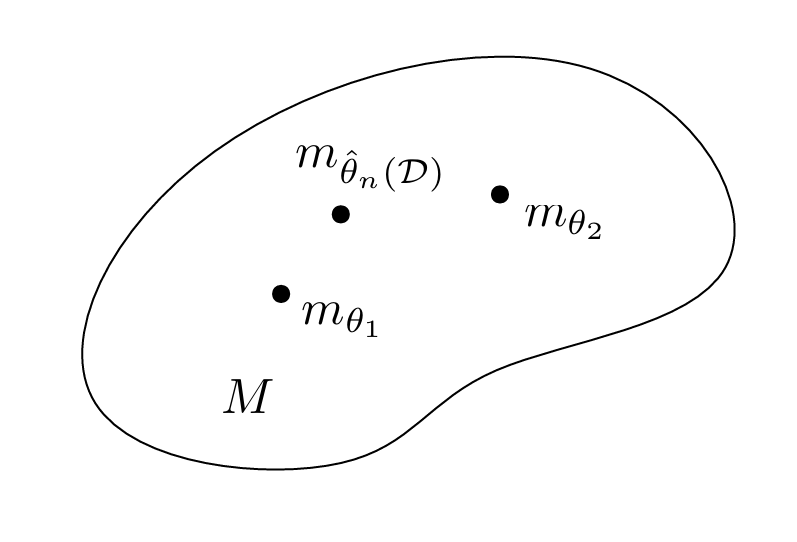
\includegraphics[width=0.5\textwidth]{Pictures/Q1/1.png}
    \caption{یک مجموعه پارامتری از توزیع‌ها}
\end{figure}\\
برای اینکه مثالی از این موضوع بزنیم می‌توانیم به مجموعه زیر اشاره کنیم:\\
\begin{equation}
    \mathcal{P}=\left\{ p_\lambda(x)=\frac{1}{\sqrt{2\pi \sigma^2}}\exp\left(-\frac{(x-\mu)^2}{2\sigma^2}\right),\ \lambda=(\mu,\sigma)\in \mathbb{R}\times \mathbb{R}_{++} \right\}
\end{equation}\\
که نشان دهنده مجموعه توزیع‌های گوسی تک‌ متغیره است. در اینجا $\lambda$ پارامتر توزیع‌ است که شامل میانگین و انحراف معیار توزیع گوسی است. اما به صورت معادل این مجموعه را به صورت‌های دیگر(با پارامترهای دیگر) نیز می‌توان نمایش داد. برای مثال داریم:
\begin{equation}
    \mathcal{P}=\left\{p_{\lambda'}(x)=\frac{1}{\sqrt{2\pi\lambda_2'}}\exp\left(-\frac{(x-\lambda'_1)^2}{2\lambda_2'}\right), \lambda'=(\mu, \sigma
    ^2)\in\mathbb{R}^2\right\}
\end{equation}\\
و همینطور:
\begin{equation}
    \mathcal{P}=\left\{p_{\lambda''}(x)=\frac{1}{\sqrt{2\pi}e^{\lambda_2''}}\exp\left(-\frac{(x-\lambda_1'')^2}{2e^{2\lambda_2''}}\right), \lambda''=(\mu, \log(\sigma))\in\mathbb{R}^2\right\}
\end{equation}\\
که اگر با پارامترهای گفته شده بخواهیم این مجموعه را نمایش دهیم به صورت زیر می‌باشد:\\
\begin{figure}[h!]
    \centering
    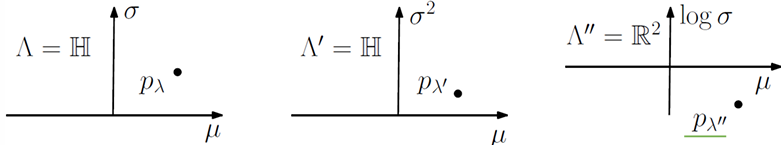
\includegraphics[width=0.7\textwidth]{Pictures/Q1/2.png}
    \caption{نمایش مجموعه یکسان با پارامترهای متفاوت(در اینجا $\mathbb{H}=\mathbb{R}\times \mathbb{R_{++}}$)}
\end{figure}\\
همانطور که از شکل‌ها مشخص است برای پارامتربندی‌های متقاوت به شکل‌های متفاوت می‌رسیم.\\
\\
حالا اگر به هندسه خمینه‌ها(منیفلدها) نگاه کنیم می‌بینیم که با اتفاق مشابهی روبه‌رو هستیم. یک منیفلد خودش یک موجود مجرد است که برای تحلیلی کردن و کار کردن با آن از نگاشت‌هایی از منیفلد به اعداد حقیقی استفاده می‌کنیم و عملا آن را پارامتریزه می‌کنیم تا بتوانیم با پارامترهای آن که اعداد هستند به راحتی کار کنیم. در اینجا نیز به طرق مختلفی می‌توان پارامتریزه کردن را انجام داد و این‌ها ماهیت خود منیفلد را تغییر نمی‌دهند. برای یک مثال ساده می‌توان به منیفلد $\mathbb{R}^2$ نگاه کرد:
\begin{figure}[h!]
    \centering
    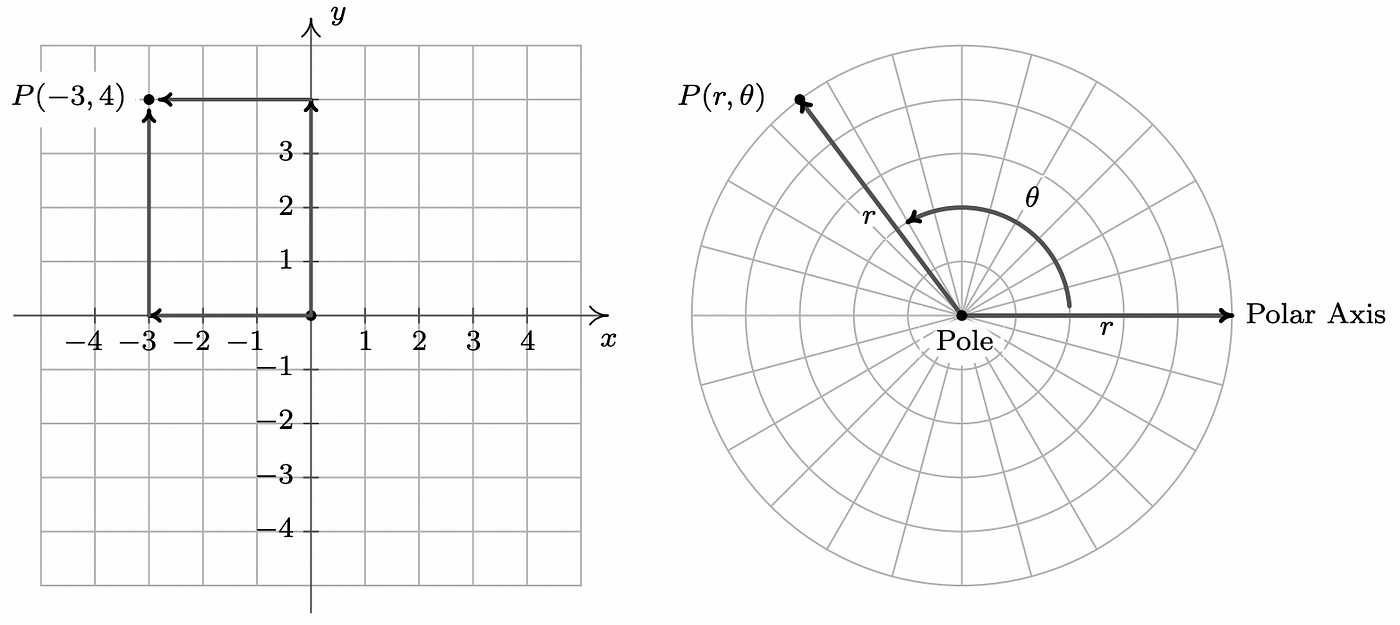
\includegraphics[width=0.6\textwidth]{Pictures/Q1/3.png}
    \caption{دو پارامتربندی مختلف از یک خمینه}
\end{figure}\\
در شکل‌های بالا دو پارامتربندی مختلف از یک خمینه را می‌بینیم. یک بار خمینه $\mathbb{R}^2$ را با مختصات دکارتی پارامتریزه یا مخصته بندی می‌کنیم و یک بار با مختصات قطبی. البته اگر بخواهیم دقیق باشیم استفاده از مختصات قطبی برای پارامتریزه کردن کل منیفلد کمی ایراد دارد از آنجایی که برای هر نقطه که زاویه $\theta$ داشته باشد می‌توان $\theta+2k\pi$ را نیز به آن نقطه نسبت داد که این با تعریف منیفلد که در قسمت بعدی ارایه می‌کنیم مطابقت ندارد. یک راهکاری که برای حل این مشکل مخصات قطبی به نظر می‌رسد مفید باشد این است که بازه زاویه را $[0,2\pi)$ در نظر بگیریم اما این هم به علت ناپیوستگی‌ای که ایجاد می‌شود مناسب نیست, همچنین در مبدا همچنان با این مشکل مواجه هستیم چون هر زاویه‌ای می‌توانیم به آن نسبت دهیم.